\documentclass[a4paper,12pt,oneside]{book}

\usepackage[pdftex]{graphicx}
\graphicspath{ {./images/} }

\usepackage{biblatex}
\addbibresource{bibliography.bib} 

\usepackage{amsthm} % definicje

\theoremstyle{definition}
\newtheorem{definition}{Definicja}
\newtheorem*{formal}{Definicja formalna}

\usepackage{pdfpages}

\usepackage{indentfirst} % akapity

\usepackage{lipsum}

\usepackage{polski}
\usepackage[T1]{fontenc}

\usepackage[pdftex,
            left=1in,right=1in,
            top=1in,bottom=1in]{geometry}

\usepackage{fancyhdr} % headers

\pagestyle{fancy}
\renewcommand{\sectionmark}[1]{\markright{\thesection\ #1}}
\fancyhead{}
\fancyhead[HR]{\thepage}
\fancyhead[HL]{\rightmark}
\setlength{\headheight}{15pt}
\fancyfoot{}

\begin{document}


\includepdf{titlepage.pdf}

\tableofcontents{}

\chapter*{Wstęp}
\addcontentsline{toc}{chapter}{Wstęp}

 Graficzny interfejs użytkownika (ang. graphical user interface, \textbf{GUI}) jest typem interfejsu za pomocą którego użytkownik wchodzi w interakcję z komputerem, programem. Dobrze przemyślony, wygodny, niezawodny, pomagający użytkownikowi interfejs napewno poszerza grono użytkowników aplikacji, co może m.in dobrze wpłynąć na rozwój biznesu lub suksec twórcy. Wyobraźmy, na przykład, co by było gdyby systemy operacyjne nie miały interfejsów graficznych? Brak interfejsu bardzo podwyższa poziom przygotowania dla korzystania z takiej / takiego aplikacji / programu. Interfejsy, w większości, robią skomplikowane programy dostępnymi dla wielu ludzi. Niskopoziomowe staje się wysokopoziomowym. Interfejsy graficzne są bardzo ważną częścią każdej aplikacji. Często patrząc tylko na wizualny wygląd już nie chce z niej korzytać. To jest źle, dla niektórych użytkowników to może być bardzo krytyczne i oni pójdą szukać inne rozwiązania, szkoda, bo ze względu na funkcjonalność aplikacja może być bardzo bogata. Dlatego jest bardzo ważne dbać o to, żeby aplikacja była nie tylko funkcjonalna, ale i nie było lagów, była atrakcyjna, wygodna, dostępna.

\chapter{Wprowadzenie}

\section{CNF}

\begin{definition}[CNF]
     Koniunkcyjna postać normalna (ang. conjunctive normal form) danej formuły logicznej to równoważna jej formuła zapisana w postaci koniunkcji klauzul. Klauzula jest zbiorem literałów połączonych alternatywą. Literałem nazywamy pojedynczą zmienną zdaniową lub pojedynczą zanegowaną zmienną zdaniową. Zmienna zdaniowa to zmienna która może przyjmować wartość \textit{true} lub \textit{false} 
\end{definition}

Przykład klauzuli:

\begin{center}
    $(x \lor y \lor z)$. 
\end{center}

Przykłady literałów:

\begin{center}
    $p, q, \neg p$
\end{center}

\begin{formal}
    Formuła $\psi$ jest w koniunkcyjnej postaci normalnej jeśli jest ona koniunkcją klauzul, z których każda jest alternatywą \textit{literałów}, tzn. ma następującą postać: 
    \begin{center}
    $(p_{11} \lor p_{12} \lor \ldots \lor p_{1{k_1}}) \land (p_{21} \lor p_{22} \lor \ldots \lor p_{2{k_2}}) \land \ldots \land (p_{n1} \lor p_{n2} \lor \ldots \lor p_{n{k_n}})$
    \end{center}
    gdzie każde $p_{ij}$ jest literałem.
\end{formal}

Każdą formułę logiczną można przedstawić równoważnie w postaci CNF. Dla jednej formuły logicznej może istnieć kilka równoważnych jej formuł w CNF.  

\section{Problem spełnialności formuł logicznych}

\textbf{Problem spełnialności formuł logicznych} jest ważym problemem obliczeniowym w teorii złożoności. Wejściem problemu jest formuła logiczna w postaci CNF. Problem polega na znalezieniu wartościowania, tzn. wartości wszystkich zmiennych zdaniowych, takich, kiedy formuła staje się prawdziwa. Formułę, która posiada takie wartościowanie nazywamy formułą \textit{spełnialną} (ang. satisfiable), a która nie, odpowiednio \textit{niespełnialna} (ang. unsatisfiable).

Na przykład, formuła
\begin{center}
    $(x_1 \lor \neg x_3) \land (x_2 \lor x_3 \lor \neg x_1)$
\end{center}

jest spełnialna, dlatego, że istnieje wartościowanie które ją spełnia, np.:
\begin{center}
    $x_1 = false, x_2 = false, x_3 = false$
\end{center}

\section{SAT-solvery}

\textbf{SAT-solver} jest programem mający na celu rozwiązanie problemu spełnialności. Na wejściu program przyjmuje formulę w postaci CNF, a na wyjściu zwraca odpowiedź, czy podana formuła jest lub nie jest spełnialna. Oryginalny SAT-solver wymaga spełnienia \textbf{wszystkich} klauzul.

Większość SAT-solverów zwraca nie tylko informację o spełnialności, ale też przykładowe wartościowanie, jeśli formuła była spełnialna, lub minimalny zbiór niespełnialnych klauzul, jeśli formuła była niespełnialna.

SAT-solvery mają wiele udanych zastosowań w różnych dziedzinach, takich jak np. sztuczna inteligencja, automatyzacja projektowania elektronicznego (ang. Electronic Design Automation), analiza programów.

Istnieją różne rodzaje SAT-solverów, które rozwiązują inne odmiany problemu spełnialności formuł logicznych: 

\begin{itemize}
    \item MAX-SAT - szuka maksymalnej liczby klauzul, które mogą być spełnione, tzn. zadajemy pytanie ile maksumalnie klauzul z tej formuły dadzą formułę spełnialną jeśli połączymy je razem.
    \item Częściowy MAX-SAT (ang. Partial MAX-SAT) - podczas gdy klasyczny problem SAT wymaga spełnienia wszystkich klauzul, PM-SAT jest rozluźniony spełnienia tego wymogu poprzez oznaczenie niektórych klauzul jako miękkie (ang. soft), a innych jako twarde (ang. hard). Celem jest znalezienie wartościowania, które spełnia wszystkie klauzule twarde i maksymalizuje liczbę spełnionych klauzul miękkich.

\end{itemize}

\section{Format DIMACS CNF}

DIMACS CNF to format tekstowy reprezentujący formułę w koniunkcyjnej postaci normalnej. Pliki z formułami mogą być w dowolnym formacie tekstowym, ale najczęściej stosują się *.cnf lub *.txt. 

Reguły których trzeba pilnować, żeby poprawnie stworzyć plik z formułą: 

\begin{enumerate}
    \item Linie zaczynające się od znaku \textit{c} przedstawiają komentarze.
    \item Linia zaczynająca się od znaku \textit{p} jest definicją formuły i wygląda następująco: \textit{p cnf l k}. Gdzie \textit{l} i \textit{k} są liczbami dodatnimi, gdzie \textit{l} reprezentuje liczbę zmiennych formuły, a \textit{k} reprezentuję liczbę klauzul.
    \item Klauzule są umieszczane dokładnie po definicji formuły. Każda klauzula jest zakodowana jako sekwencja liczb dziesiętnych odseparowanymi spacjami.
    \item Każda linia zawiera dokładnie jedną klauzulę i ma kończyć się symbolem 0.
    \item Zostawianie pustych linii w formule nie jest dozwolone.
\end{enumerate}
Niepilnowanie tych reguł może doprowadzić do błędnych wyników lub w ogóle do unieruchomienia SAT-solvera.

Na przykład formuła w CNF

\begin{center}
    $(x_1 \lor x_2 \lor x_3 \lor x_4) \land (\neg x_1 \lor x_2) \land (x_3 \lor x_4 \lor \neg x_1) \land (x_2 \lor x_3 \lor \neg x_1)$ 
\end{center}

może być zakodowana w DIMACS CNF jako:

\begin{verbatim}
                                p cnf 4 4
                                1 2 3 4 0
                                -1 2 0
                                3 4 -1 0
                                2 3 -1 0
\end{verbatim}

\section{Cel i zakres pracy}

Celem pracy jest stworzenie wygodnego i dostępnego dla wszystkich interfejsu graficznego dla oryginalnego SAT-solvera. Dostępność zapewnijmy tworząc aplikację webową dlatego, że nie wymaga od użytkownika żadnych nipotrzebnych instalacji, działa prawie wszędzie i dla uruchomienia potrzebny jest tylko komputer i internet. Wygodność zapewnijmy przemyślonym interfejsem, który będzie w razie problemów pomagał użytkownikowi w ich rozwiązaniu za pomocą odpowiednich komunikatów i sugestii. W pracy zostanie omówniony proces projektowania interfejsu oraz szczegóły implementacji niektórych, najbardziej interesujących części aplikacji. 

Frontend będzie stworzony za pomocą biblioteki \textbf{React}, a backend za pomocą frameworku \textbf{FastAPI}. Na backendzie wykorzystamy pakiet \textbf{PySAT}, który daję możliwość korzystania z wielu zaimplementowanych SAT-solverów. Komunikację pomiędzy backendem a frontendem zapewnijmy poprzez HTTP zapytania.

\chapter{Projekt}

\section{Definicja funkcjonalności}

Wygląd interfejsu graficznego mocno zależy od tego, jak zdefiniujemy funkcjonalności, więc zanim zacznimy, mamy je ściślie zdefiniować.  

Mamy mieć edytor plików DIMACS CNF który będzie pomagał nam wykrywać błędy w formułach. Można wyróźnić wystąpinie następnych błędów:

\begin{itemize}
    \item \textit{Kod błędu 0}: Nie można zostawiać pustych linii
    \item \textit{Kod błędu 1}: Definicja formuły może być niepoprawna
    \item \textit{Kod błędu 2}: Każda klauzula ma kończyć się zerem
    \item \textit{Kod błędu 3}: Klauzula może być niepoprawna
    \item \textit{Kod błędu 4}: W pliku nie może być więcej niż jedna definicji formuły
    \item \textit{Kod błędu 5}: Zmienna w klauzuli może być nie w zakresie zdefiniowanym w definicji
\end{itemize}

\noindent Dla każdego z wymienionych błędów mamy dawać użytkownikowi indywidualne sugestie do poprawienia:

\begin{itemize}
    \item \textit{Kod błędu 0}: usuwanie lub edycja linijki
    \item \textit{Kod błędu 1}: edycja linijki z definicją
    \item \textit{Kod błędu 2}: dopisywane zera na końcu linijki
    \item \textit{Kod błędu 3}: usuwanie lub edycja linijki z klauzulą
    \item \textit{Kod błędu 4}: wymiana istniejącej lub usuwanie linijki z definicją
    \item \textit{Kod błędu 5}: edycja linijki z klauzulą
\end{itemize}

Błędów może być dużo, więc damy też możliwość do automatycznego poprawiania formuły. Przy tym w formule następują następne zmiany:

\begin{enumerate}
    \item Na końcach linii są dopisywane zera.
    \item Liczby zmiennych i klauzul w nagłówku są poprawiane na odpowiednie.
    \item Puste linie i niepoprawne klauzule są usuwane.
    \item Komentarze są usuwane.
\end{enumerate}

\noindent Ze względu na to, że formuła może być nieostrzożnie uszkodzona, użytkownik będzie poproszony o potwierzdzenie chęci zrobienia automatycznego poprawienia.

Ma istnieć możliwość do wczytania formuły w postaci DIMACS CNF z pliku oraz zapisywania do pliku.

Formuła z edytora ma być parsowana do zwykłej postaci CNF. W tej postaci formułę można będzie modyfikować, czyli usuwać, zmieniać lub dodawać klauzule. Dzięki temu użytkownik dostanie możliwość jednoczesnej edycji formuły w postaci CNF i DIMACS, może zanim wybrać wygodniejszy dla siebie sposób pracy z programem.

Korzystając z SAT-solvera użytkownik ma możliwość:

\begin{itemize}
    \item znalezienia i wyświetlenia pojedynczego wartościowania spełniającego formułę
    \item możliwość znalezienia i wyświetlenia wszystkich wartościowań spełniających
    \item wybrać SAT-solver z którego chce korzystać
\end{itemize}

Reszta:

\begin{itemize}
    \item wyświetlanie ilości znalezionych rozwiązań
    \item zapisywanie pojedynczego wartościowania w postaci czytelnej dla komputera, czyli zero-jedynkowo
    \item możliwość usuwania zduplikowanych klauzul z formuły
    \item możliwość lączenia dwóch formuł w jedną, co z kolei daje możliwość lączenia dowolnej ilości formuł
\end{itemize}

\section{Prototypowanie interfejsu}

W zakresie prototypowania komponent po komponencie stworzymy prototyp graficznego interfejsu SAT-solvera oraz rozważymy przyjęte decyzji projektowe.

\subsection{Edytor plików w formacie DIMACS CNF}

Korzytając z SAT-solverów jesteśmy zmuszeni korzystać z plików w formacie DIMACS CNF, więc przydałoby się mieć edytor do takich plików. W podstawowej wersji będzie wyglądał następująco:

\newpage

\begin{figure}[ht]
    \centering
    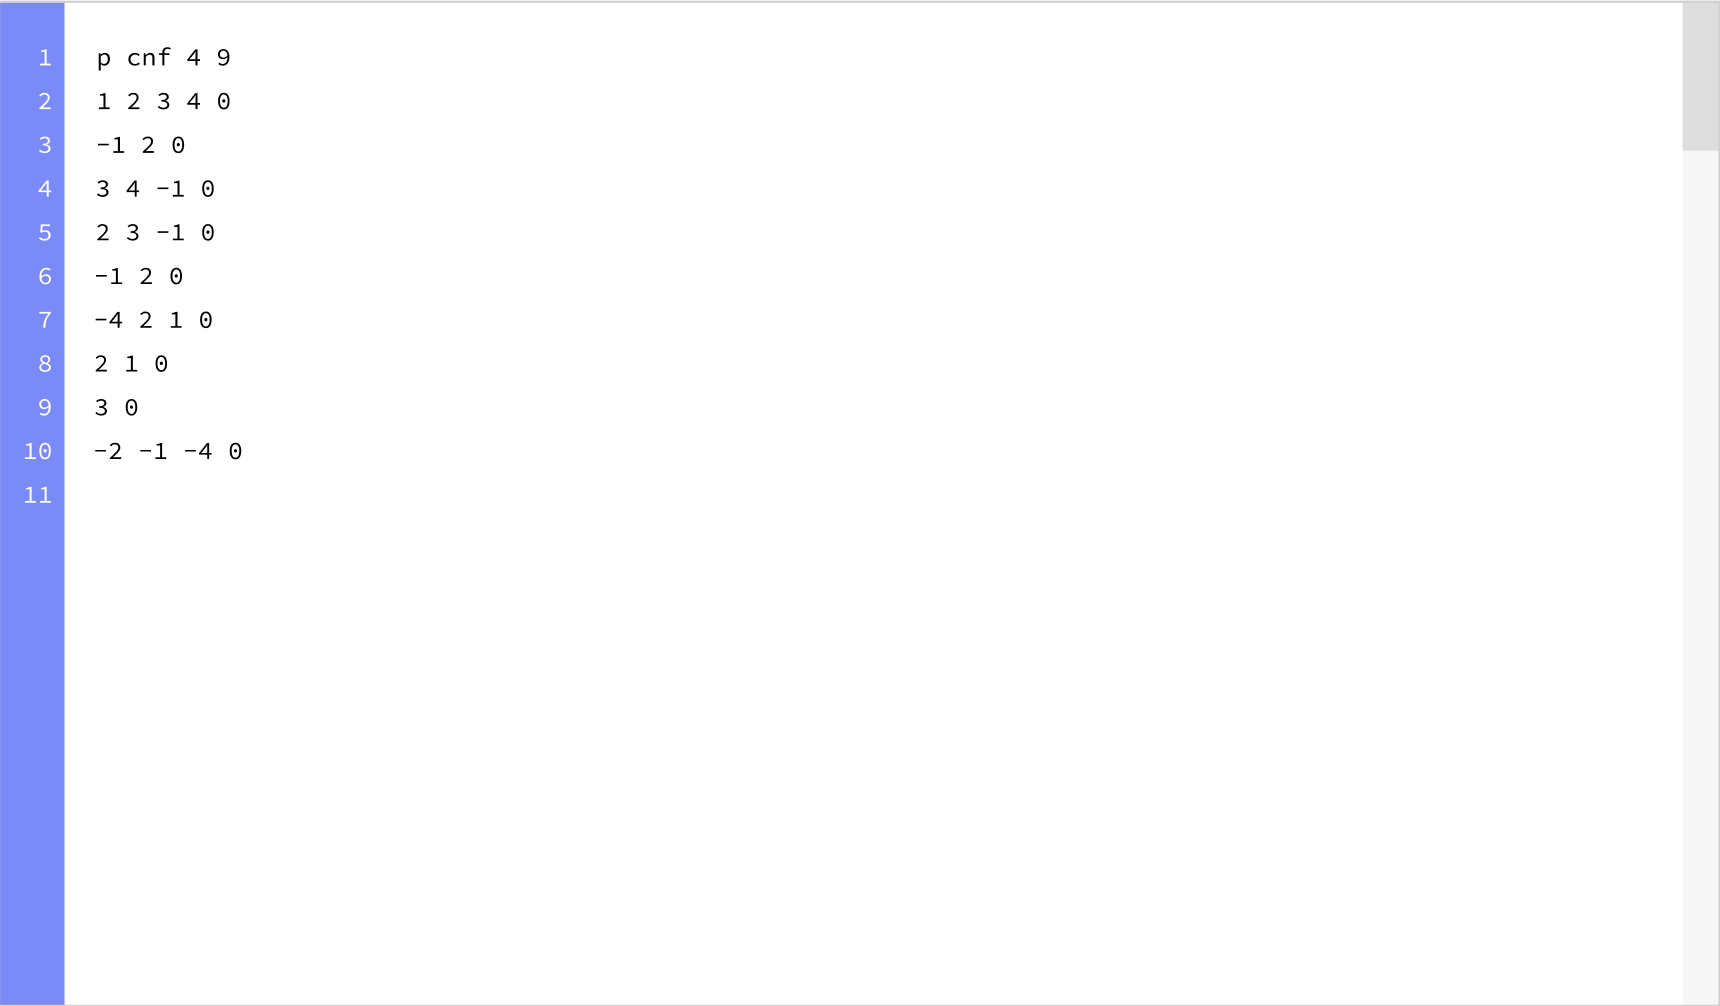
\includegraphics[width=14.30cm]{1}
    \caption{Edytor podstawowy}
    \label{fig:1}
\end{figure}

\noindent W środku większą częsć zajmuje obszar w którym będziemy modyfikować naszą formułę, na razie istnieje możliwość tylko wklejenia jej do edytora. Po prawej stronie mamy scroll który będzie pomagał nam przemieszczać się po formułach z dużą liczbą klauzul. Po lewej stronie mamy słupek z informacją o numerach linii, w przyszłości nam się to przyda dla wykrycia i wskazywania błędów.

Nie za bardzo wygodne jest wklejanie zawartości pliku, więc damy użytkownikowi możliwość do załadowania pliku z formułą oraz możliwość do zapisania pliku z zmodyfikowaną formułą:

\newpage

\begin{figure}[ht]
    \centering
    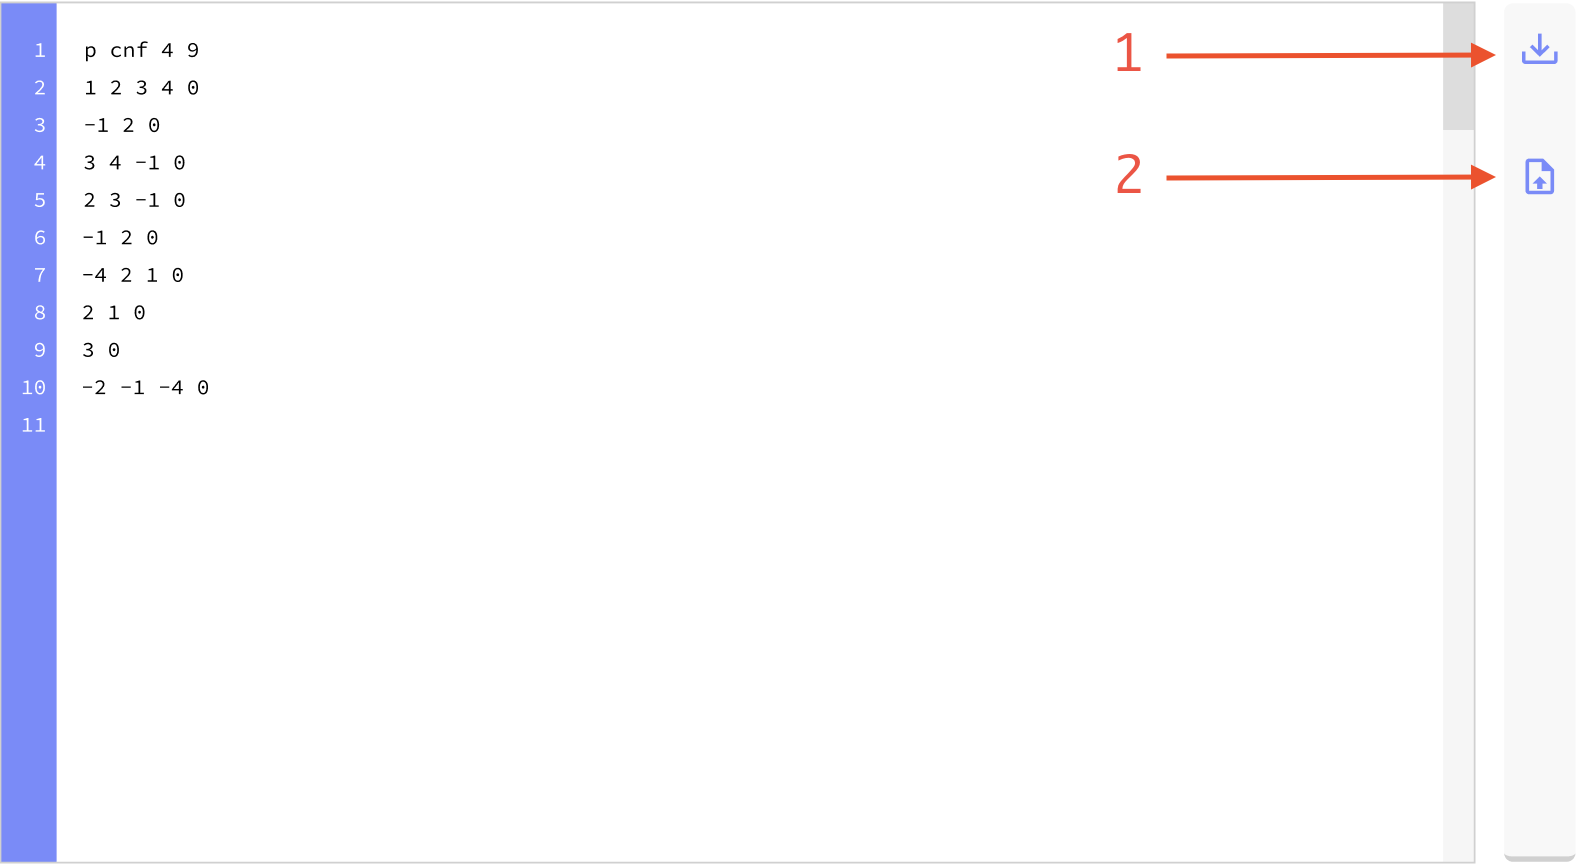
\includegraphics[width=14.30cm]{2}
    \caption{Edytor z możliwością załadowania i zapisania formuły}
    \label{fig:2}
\end{figure}

\noindent Po prawej stronie dodaliśmy obszar który będzie pomagał nam zarządzać edytorem, obecnie znajdują się tu dwa przyciski: nr. 1 daje możliwość wybrać i załadować plik z formułą, a nr.2 daje możliwość zapisać plik i dać mu nazwę.

W formule, przez przypadek, mogą pojawić się zduplikowane klauzule, chociaż to nie za bardzo wpływa na wydajność i szybkość działania SAT-solvera, damy użytkownikowi możliwość usunięcia takich klauzul:

\begin{figure}[ht]
    \centering
    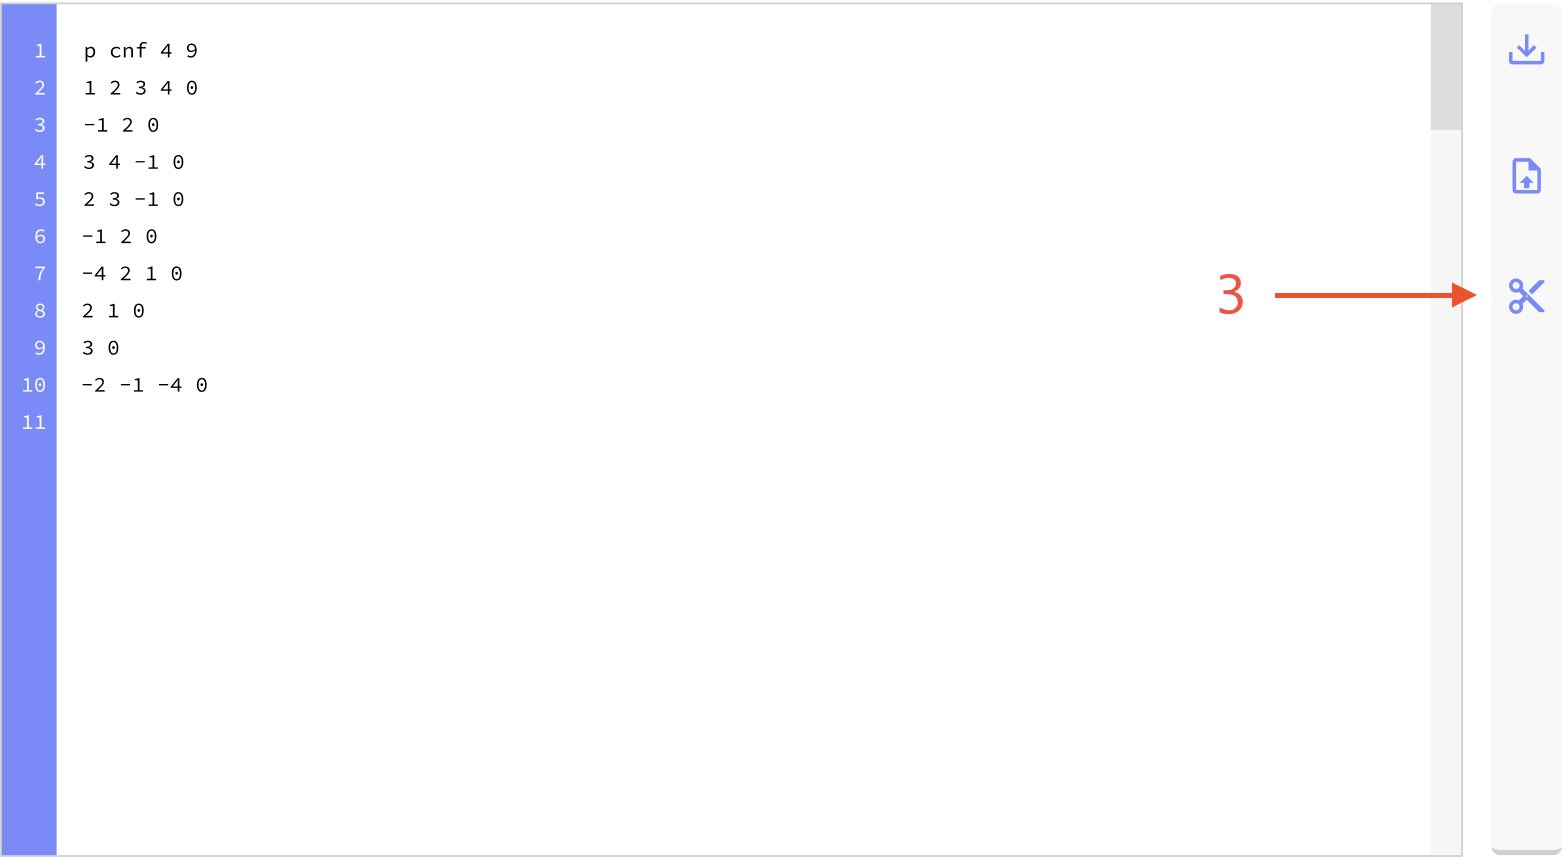
\includegraphics[width=14.30cm]{3}
    \caption{Edytor z możliwością usunięcia zduplikowanych klauzul}
    \label{fig:3}
\end{figure}

Z obrazów przycisków z obszaru do zarządzania edytorem może nie być jasne, co one robią, więć dodana jest możliwość zobaczyć w postaci tekstowej tę informację. Przy najechaniu myszką na każdy z przycisków pod nimi będzie pojawiała się podpowiedź (ang. tooltip) z tekstem. Na przykład pod przyciskiem nr.1 pojawi się komunikat "Upload formula".

\newpage

\subsection{Wykrycie, wskazywanie i naprawienie błędów}

Dla poprawnego i przewidywanego działania SAT-solvera konieczne jest poprawne stworzenie pliku z formułą w formacie DIMACS CNF. Jako twórcy interfejsu graficznego mamy pomoc użytkownikowi poradzić z wykryciem, wskazywaniem i naprawieniem błędów w razie ich wystąpienia. 

Kiedy formuła w edytorze będzie się zmieniała, będzie wywoływana funkcja wykrywająca błędy. Wykryte błędy mamy w jakiś sposób wyświetlić. Propnujemy podświetlenie odpowiednich linijek. Tak to będzie wyglądało: 

\begin{figure}[ht]
    \centering
    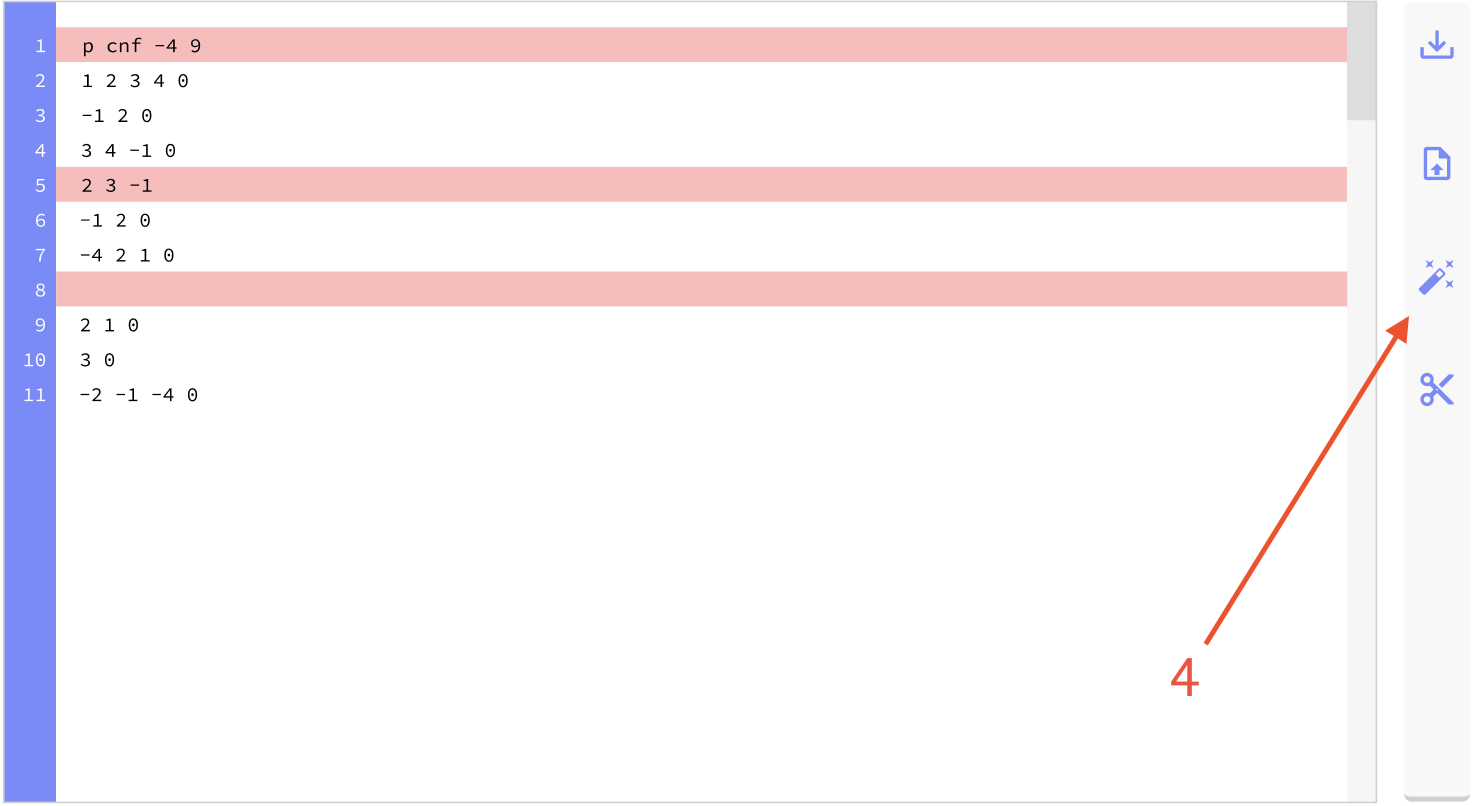
\includegraphics[width=14.30cm]{4}
    \caption{Edytor wraz z tabelą z błędami}
    \label{fig:4}
\end{figure}

\noindent Widzimy jeszcze, że w obszar do zarządzania formułą został dodany nowy przycisk pod numerem 4. Będzie on odpowiadał za automatyczne poprawienie błędów. Kiedy użytkownik nacisnie na ten przycisk, zanim poprawienie się zacznie, będzie wyświetlony komunikat mówiący o bezzwrotności działań użytkownika i prośbą o potwierdzenie chęci zrobienia popraw. Dodatkowo w komunikacie będzie napisano, że: 

\begin{itemize}
    \item puste linie, komentarze oraz uszkodzone klauzule zostaną usunięte
    \item liczba zmiennych i klauzul będzie przeliczona
\end{itemize}

W tym momencie, jeśli użytkownik będzie miał błędy w formule, będzie je dobrze widział, ale ma je też naprawić. Żeby to teraz zrobić, ma z góry wiedzieć w czym jest problem. Ułatwmy zrozumienie dodaniem odpowiednich podpowiedzi przy najechaniu myszką na czerwoną linię. Na rysunku 2.5 pojawiła się podpowiedź, gdzie w pierwszej linijce znajduje się treść uszkodzonej linii, w drugiej opis błędu, a w trzeciej propozycja do naprawienia w postaci przycisku. W tym przykładzie widzimy, że zapropanowano dodnie zera na końcu linii.

\begin{figure}[ht]
    \centering
    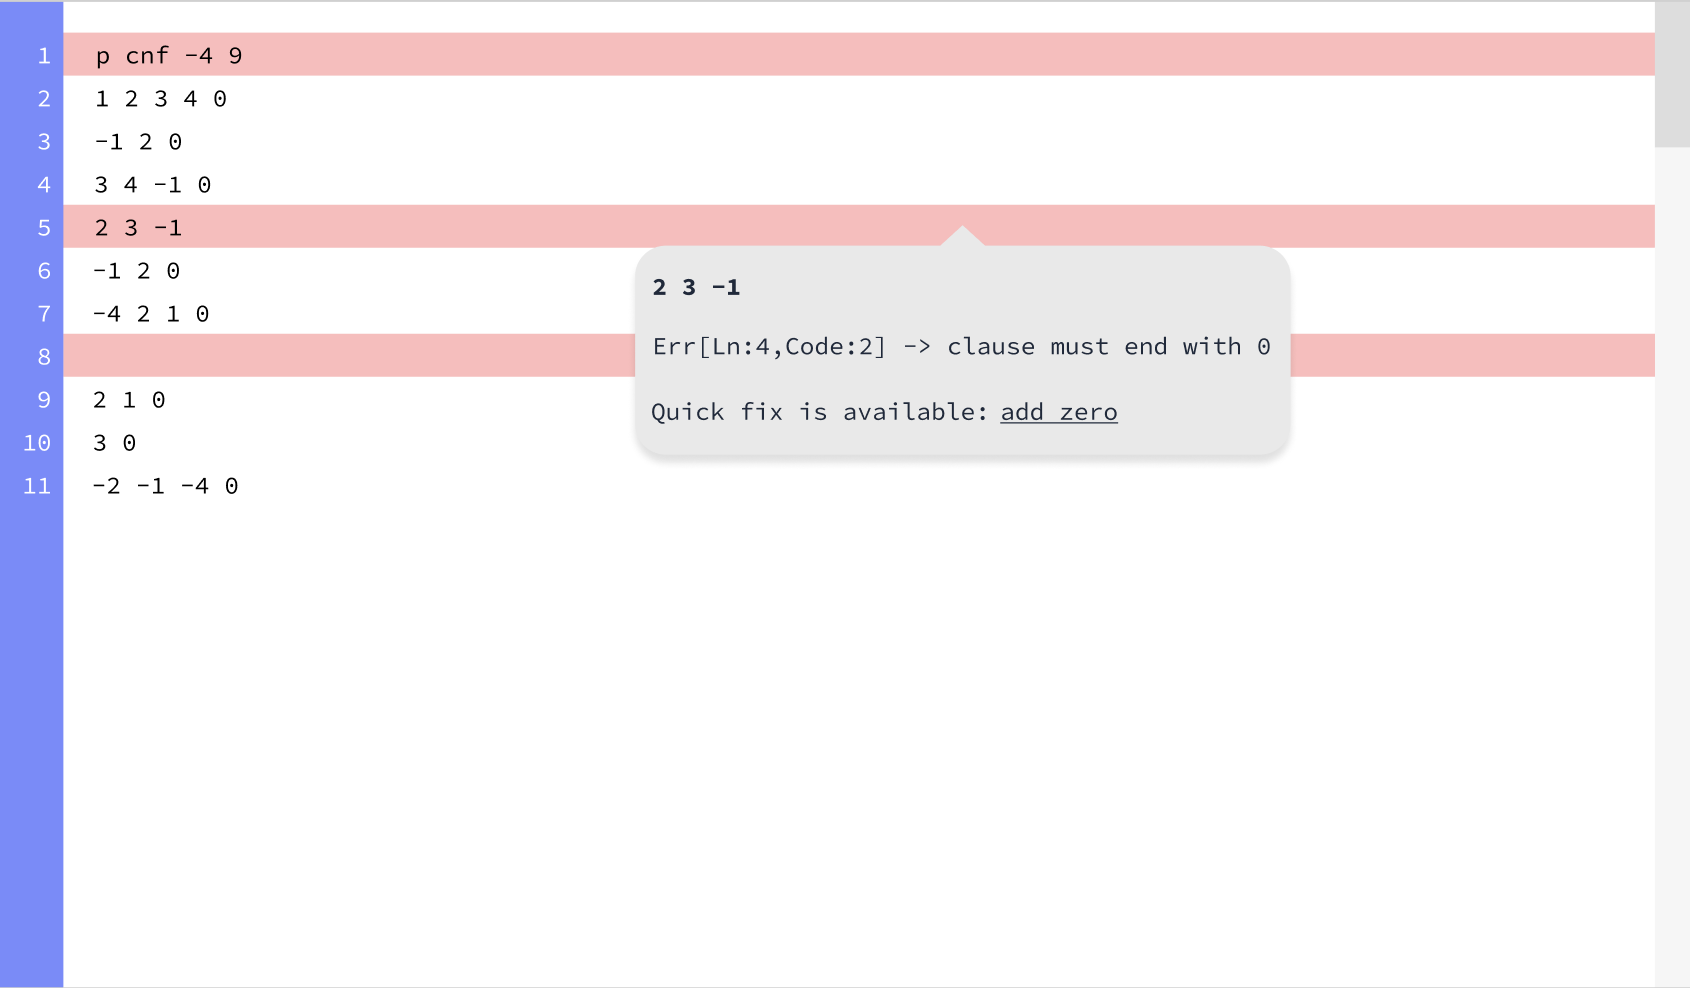
\includegraphics[width=14.30cm]{5}
    \caption{Edytor wyświetlający podpowiedź przy najechaniu myszką}
    \label{fig:5}
\end{figure}

\newpage

Zostały nam jeszcze dwa problemy do rozwiązania. Po pierwsze, w razie błędów nie widzimy od razu ile ich jest. Po drugie, ze względu na to, że pliki z formułami mogą zawierać dużo klauzul, a zatem potencjalnie dużo błędów, nie mamy sposóbu na wyświetlanie wszystkich blędów naraz w jednym miejscu. W drugim przypadku przydało by się też zostawić możliwość szybkiej naprawy. 

Te dwa problemy można rozwiązać wprowadzając kolejny komponent, który będzie znajdował się od razu pod edytorem: 

\begin{figure}[ht]
    \centering
    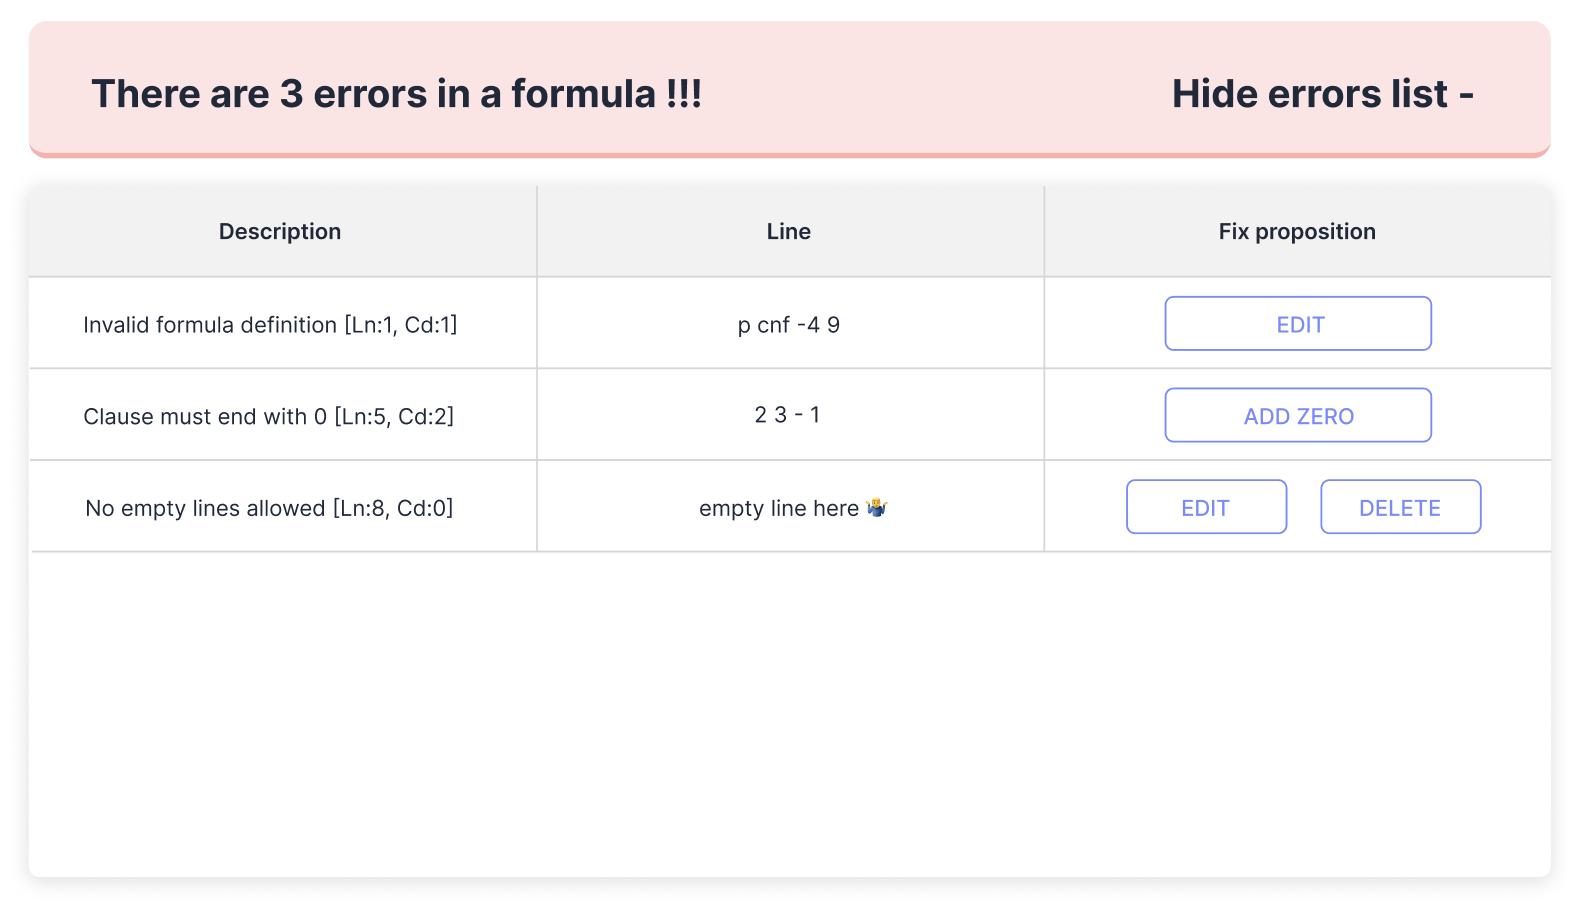
\includegraphics[width=14.30cm]{6}
    \caption{Tabela z wykrytymi błędami}
    \label{fig:6}
\end{figure}

\noindent Jest ukryty, kiedy formuła nie zawiera błędów. Ma dwa stany: otwarty i zamknięty. Domyślnie ma stan zamknięty. Na górze widzimy nagłówek w którym jest napisano ile mamy błędów w formule. Klikająć na nagłówek zmieniamy stan otwarcia. Tabela ma trzy kolumny: w pierwszej znajduje się opis błędu, w drugie uszkodzona linia, a w trzeciej znajdują się przyciski, dzięki którym można szybko naprawić błąd. Błędy w tabeli są sortowane rosnąco w zależności od indexu linii wystąpienie.

\subsection{Podstawowe funkcje SAT-solvera}

Kiedy umiemy już wykrywać i naprawiać błędy, co zapewnia nam bezpieczne i przewidywane działania SAT-solvera, możemy dodać przyciski kontrolujące i dać użytkownikowi możliwość do uruchomienia go:

\begin{figure}[ht]
    \centering
    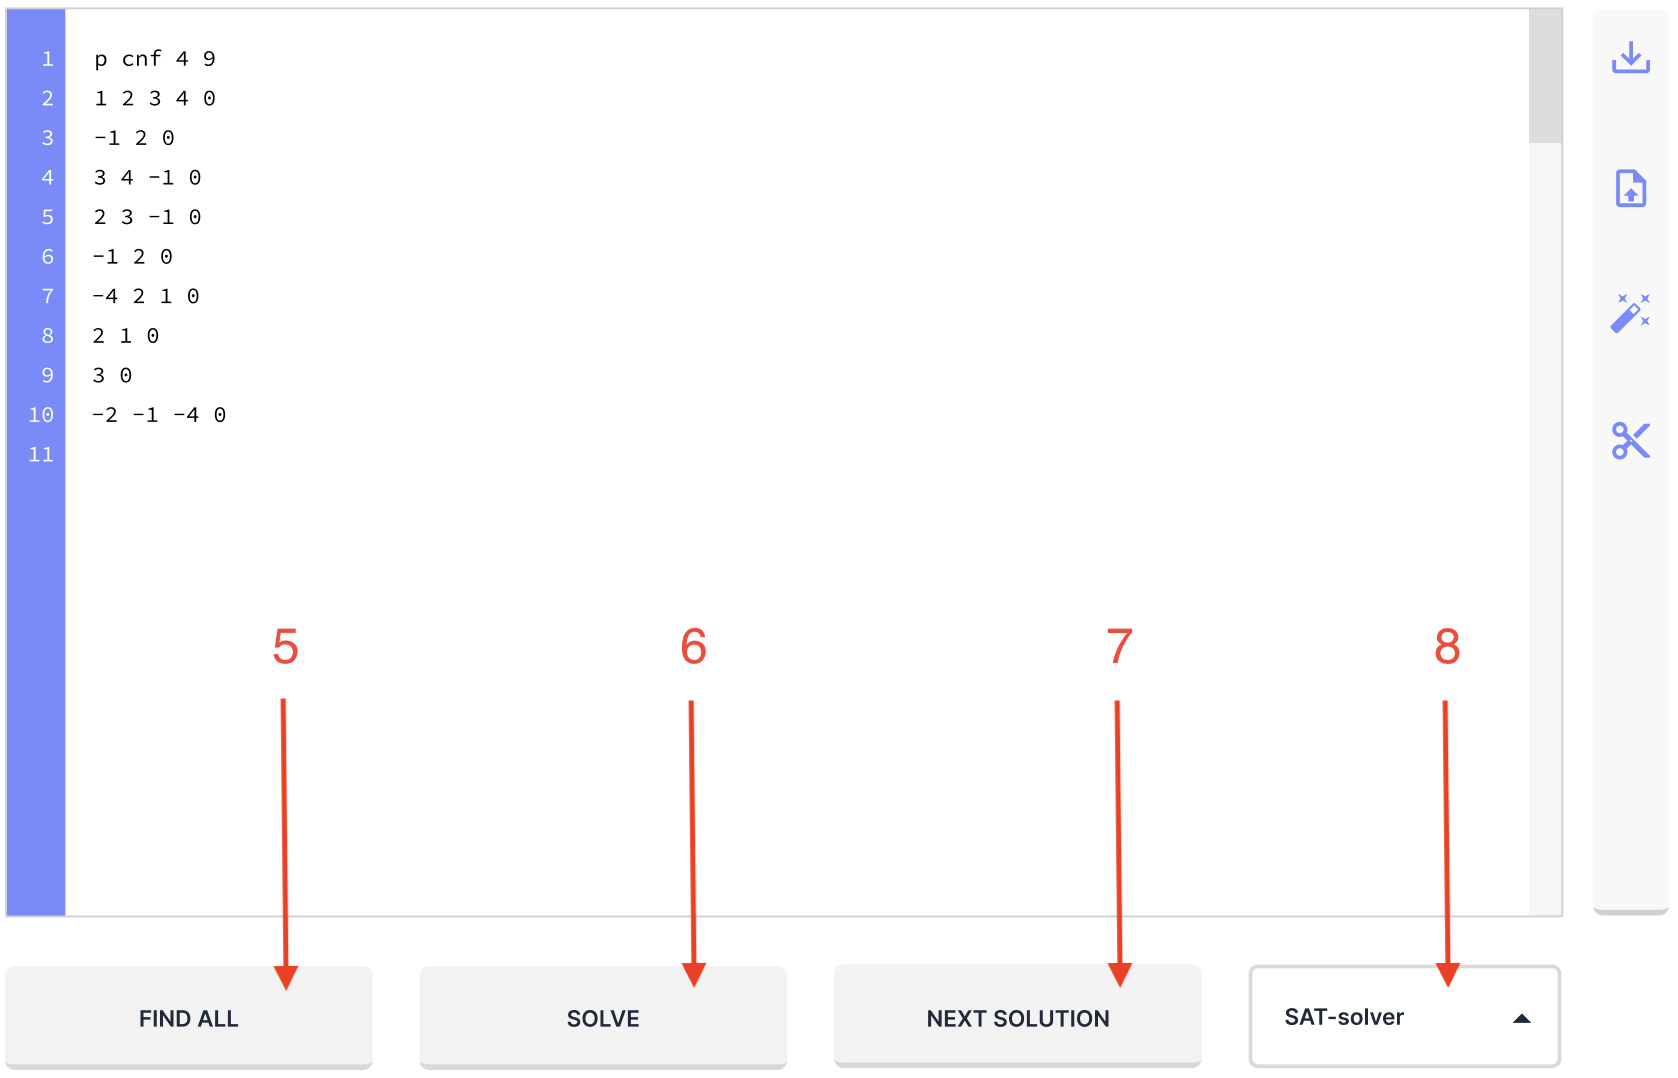
\includegraphics[width=14.30cm]{7}
    \caption{Edytor ze wszystkimi przyciskami}
    \label{fig:7}
\end{figure}

Przycisk nr.6 pozwala dowiedzieć czy formuła jest lub nie jest spełnialna. Jeśli jest spełnialna zwracane jest pierwsze wartościowanie.

Przycisk nr.7 pozwala znaleźć następne wartościowanie, jeśli takie istnieje. Jest nieaktywny jeśli formula jest niespełnialna.

Przycisk nr.5 uruchamia wyszukiwanie wszystkich wartościowań. Wyszukiwanie można będzie przerwać w dowolnej chwili kiedy będzie znalezione pierwsze wartościowanie. Po przerwaniu wyszukiwanie można ponownie zacząć od momentu skończenia, w tym przypadku tekstem przycisku będzie nie "FIND ALL", a "FIND OTHER SOLUTIONS".

Przycisk nr.8 pozwala wybrać dowolny z dostępnych w pakiecie PySAT SAT-solver.

Jeśli formuła w edytorze zawiera błędy - uruchomienie SAT-solvera nie jest dozwolone. Wszystkie wymienione przyciski oprócz nr.8 będą nieaktywne.

\subsection{Wyświetlanie wartościowań}

Chcemy, żeby komponent pozwalał w jasny sposób widzeć jakie wartości zostały przepisane zmiennym formuły.

Mamy poradzić z problemem wyświetalania wartościowań dla formuł zawierających dużą liczbę zmiennych. Trudno będzie wyświetlić takie wartościowanie wprost w słupku lub w jednej linii, doprowadzi to do przekroczenia granic ekranu dowolnego rozmiaru wzdłuż osi X lub Y. 

%\newpage

\subsection{Formuła w postaci CNF}

Komponent, który stworzymy, będzie dawał możliwość zoboczenia i edytowania formuły inaczej, niż w edytorze DIMACS, a mianowicie w zwykłej postaci CNF. Ważne tu jest umieszczenie wszystkiego w wygodny sposób dlatego, że formuły często zawierają dużo klauzul i to też może zająć dużo miejsa na ekranie, a im więcej umieszczamy elementów na ekranie, tym wolnejszy staje się rendering tego wszystkiego w przeglądarce. Wolne działanie aplikacji może źle wpłynąć na doświadczenie użytkownika przy korzystaniu z niej, czemu chcemy zapobiec.

Proponujemy stworzenie następnego komponentu:

\begin{figure}[ht]
    \centering
    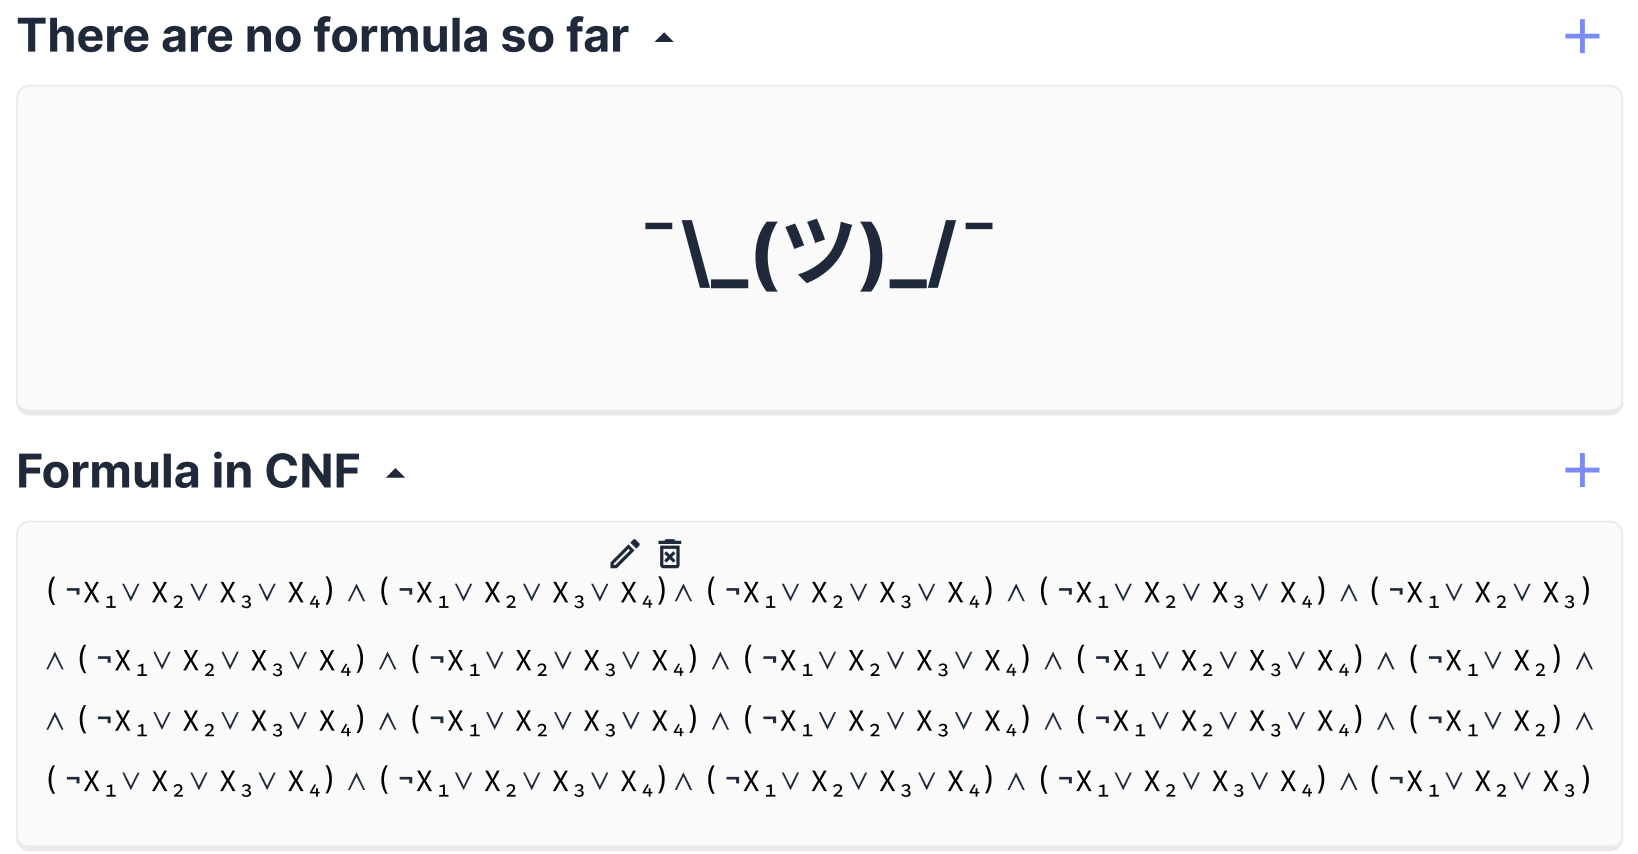
\includegraphics[width=14.30cm]{9}
    \caption{Komponent pozwalający pracować z formułą w postaci CNF}
    \label{fig:9}
\end{figure}

\noindent To wszytko to jest ten sam komponent, ale na górze znajduje się w stanie, kiedy formuła jeszcze nie została dodana. Klikając na nagółwek komponentu możemy go zamknąć lub otworzyć. Domyślnie znajduje się w stanie otwartym.

Klikając na plus możemy ręcznie dodawać klauzule do formuły. Pojawi się do tego odpowiednie pole z miejscem do stworzenia wraz z instrukcją, w której jest wytłumaczone jak to prawidłowo zrobić.

W stanie nr.2, nad drugą klauzulą widzimy przyciski pozwalające ją modyfikować. Takie przyciski będą pojawiać się nad każdą klauzulą przy najechaniu na nią myszką. Przy nacisnięciu na śmietnik użytkownik zostanie zapytany, czy napewno chce usunąć klauzule. W razie pozytywej odpowiedzi klauzula będzie usunięta. Przy nacisnięciu na długopis, użytkownik dostaje możliwość do modyfikacji zawartości klauzuli. Kiedy modyfikowanie jest skończone, naciska na przysick "Zapisz", który stanie się dostępny w interfejsie graficznym lub "Enter" na klawiaturze.

Zostało nam jeszcze poradzić z obsługą formuł zawierających dużo liczbę klauzul. Zrobimy to jak w przypadku dużej ilości wartościowań formuły, czyli rozdzielimy dane na strony. Ilość klauzul wyświetlanych na jednej strone będzie stała i znajdowała się w kodzie programu, użytkownik nie będzie w stanie jej zmieniać. Domyślnie na jednej stronie będziemy pokazywali 115 klauzul. Takie rozdzielenie dobrze wpłynie na wydajność aplikacji dlatego, że przeglądarka nie będzie miała renderować całą formułę naraz, a tylko odpowiednią jej część. Wyglądać to będzie następująco:

\begin{figure}[ht]
    \centering
    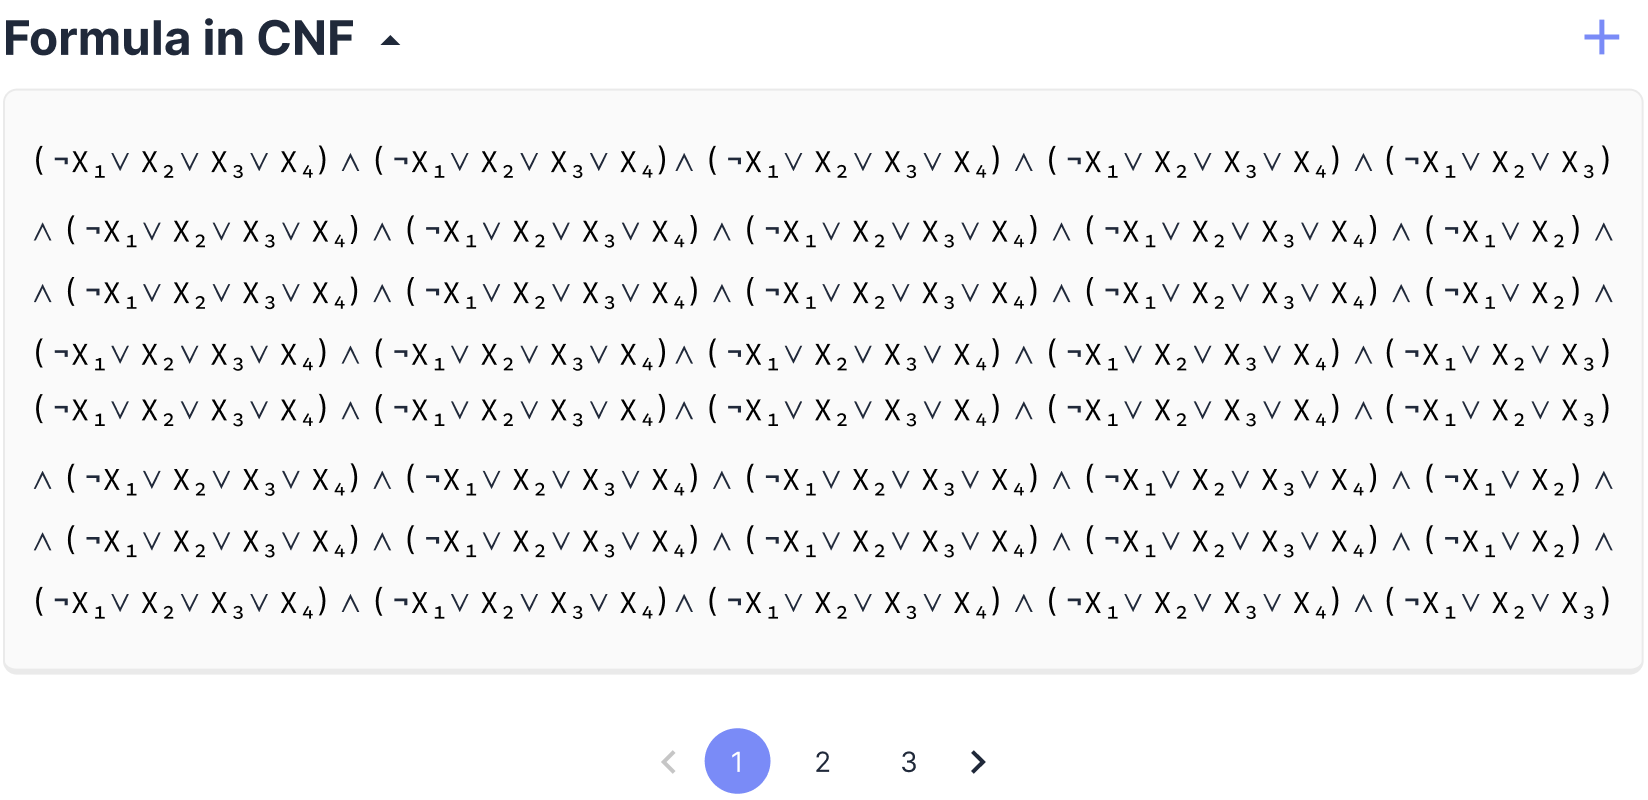
\includegraphics[width=14.30cm]{10}
    \caption{Duża formuła rozdzielona na kilka stron}
    \label{fig:10}
\end{figure}

\subsection{Łączenie formuł}

Został nam do zaprojektowania ostatni komponent, taki, który będzie pozwalał łączyć formuły w formacie DIMACS CNF, zaprojektujemy go w następny sposób: 

\begin{figure}[ht]
    \centering
    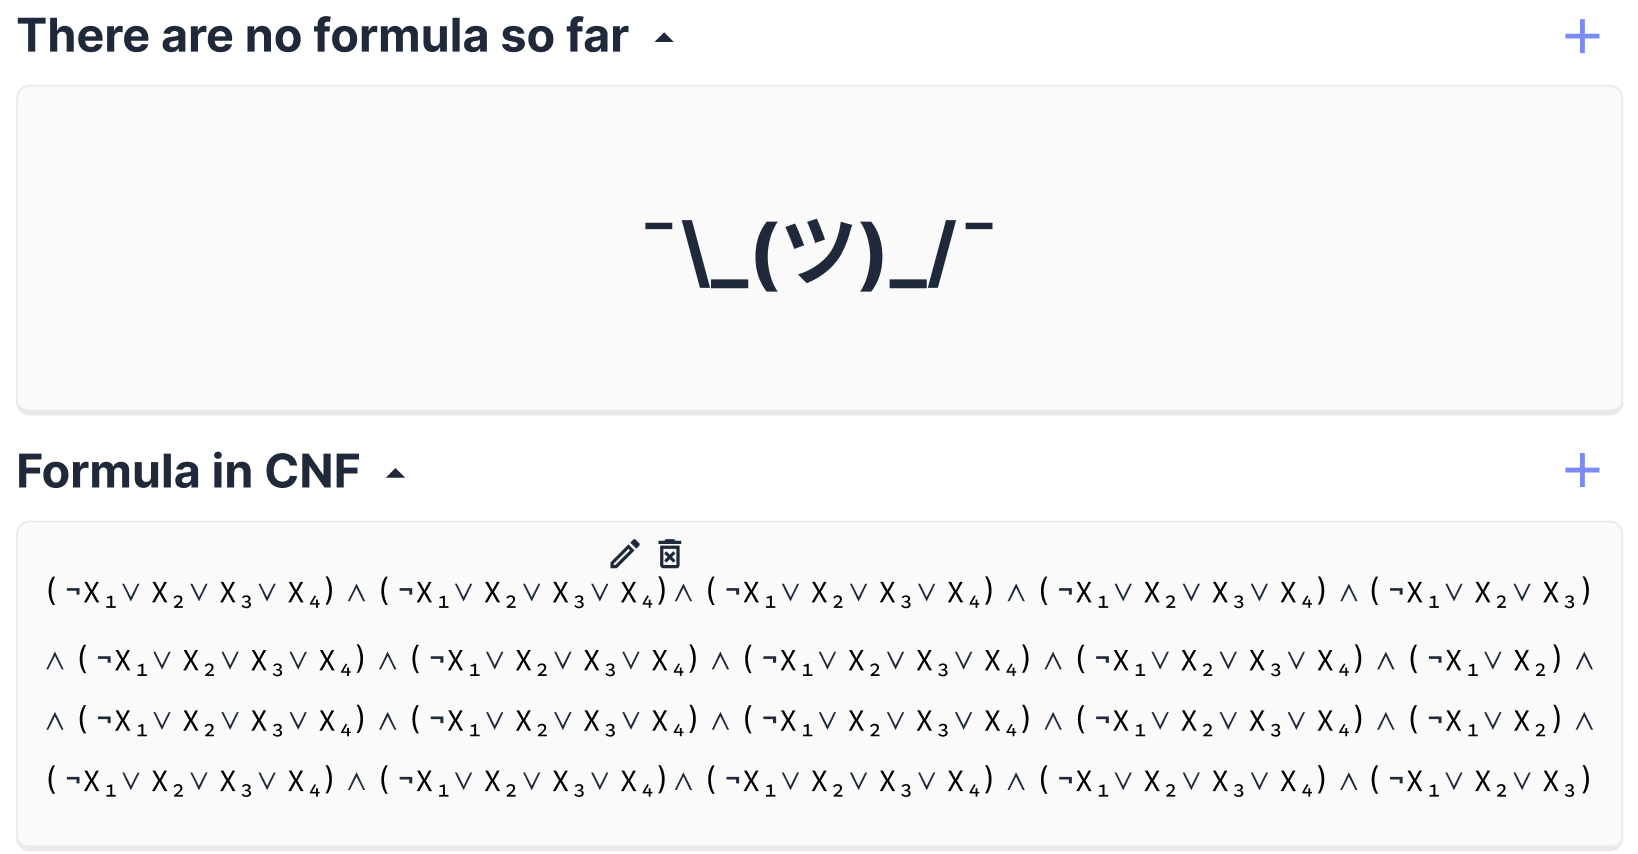
\includegraphics[width=14.30cm]{11}
    \caption{Komponent pozwalający łączyć formuły}
    \label{fig:11}
\end{figure}

\noindent Widzimy tu najpierw dwa edytory i dwa przyciski. Edytory nie mają możliwości sprawdzenia błędów. Do edytorów można wkleić lub załadować formułę z pliku, klikając na przycik nr.1 lub nr.2. Kiedy dwie formuły zostały załadowane, użytkownik może nacisnąć przycisk "LINK FORMULAS". Jeśli nie wystąpiło błędów podczas łączenia, pojawi się odpowiedni komunikat, że formuły zostały pomyślnie połączone oraz odblokuje się przycisk "PASTE RESULT IN THE EDITOR". Kiedy użytkownik kliknie na przycsik nr.4, to zostanie przekierowany na stronę z edytorem w który już będzie wklejony rezultat łączenia.

\section{Architektura aplikacji}

\lipsum[1]

\lipsum[2]

\lipsum[3]

\chapter{Implementacja}

\section{Narzędzia}

\subsection{PySAT}

Darmowa i otwarta biblioteka przeznaczona dla języka Python.

\lipsum[1]

\lipsum[2]

\lipsum[3]

\subsection{FastAPI}

Darmowa i otwarta biblioteka przeznaczona dla języka Python.

\lipsum[1]

\lipsum[2]

\lipsum[3]

\subsection{React}

Darmowa i otwarta biblioteka przeznaczona dla języka JavaScript.

\lipsum[1]

\lipsum[2]

\lipsum[3]

\section{Implementaja edytora}

\lipsum[1]

\lipsum[2]

\lipsum[3]

\section{Implementacja sprawdzarki}

\lipsum[1]

\lipsum[2]

\lipsum[3]

\section{Optymalizacje}

\lipsum[1]

\lipsum[2]

\lipsum[3]

\lipsum[4]

\chapter*{Podsumowanie}
\addcontentsline{toc}{chapter}{Podsumowanie}

Ja chcę, żeby mój program stał się początkiem tworzenia interfejsów graficznych dla różnych rodzajów SAT-solverów. Ze względu na brak takich programów. W mojej pracy dotknąłem tylko mało część, dużo rzeczy można jeszcze do tego dodać.

Będę \cite{einstein} zawsze otwarty na takie propozycję na GitHubie. Chciałbym, żeby \cite{dirac} studenci naszej uczelni w \cite{dirac} swoich pracach licencjackich lub \cite{knuthwebsite} nawet magisterskich \cite{knuth-fa} kontynuowali rozwijanie i polepszenie mojego programu.

\listoffigures{}
\addcontentsline{toc}{chapter}{Spis rysunków}

\printbibliography[title=Bibliografia]
\addcontentsline{toc}{chapter}{Bibliografia}

\end{document}
